\subsubsection{\bf Introduction}
LineTrackingMonitor is a tool to monitor various lines included in the strain data.
The amplitude and frequency are tracked.


\subsubsection{{\bf Function:} butterBandPass}
{\tt ~ butterBandPass dat fs flow fhigh order\\}
\\
This applies a Butterworth bandpass filter of given cutoff frequencies and filter order to given data.
\\
The arguments of this function are:
\begin{itemize}
\item {\tt dat}: Input. data
\item {\tt fs}: Input. Sampling frequency [Hz]
\item {\tt flow}: Input. Lower cutoff frequency [Hz]
\item {\tt fhigh}: Input. Higher cutoff frequency [Hz]
\item {\tt order}: Input. Filter order
\end{itemize}

It should be noted that this filter is a zero-phase filter (so called filtfilt), so the effective filter order is twice your input value (For example, if you set order $= 5$, the actual filter order becomes ten).


\subsubsection{{\bf Function:} nha}
{\tt ~ nha dat fs nsig nframe nshift nstart nend tlength\\}
\\
The algorithm of NHA is essentially an iteration of least-square fitting of data with a sinusoidal wave. At each iteration, it tries to minimize the following cost (error) fuction:
\begin{equation}
F(\hat{A},\hat{f},\hat{\varphi})=\frac{1}{N}\sum_{n=0}^{N-1} \left\{ x(n) - \hat{A} \cos \left(2\pi \frac{\hat{f}}{f_{s}}n+\hat{\varphi} \right) \right\}^2,
\label{eq:nha_cost}
\end{equation}
where $x(n)$ is a given discrete time signal, and the sinusoidal model signal is characterized by three parameters: amplitude $\hat{A}$, frequency $\hat{f}$, and initial phase $\hat{\varphi}$. $f_{s}$ is the sampling frequency. We cut out from the data a window of length of $N$ samples, which is called {\it frame}. Frames usually overlap each other, and we refer to the constant distance of adjacent frames as shift length. In this section, we define the time representing a given frame as follows: for the frame which starts at time $t=t_{1}$ and ends at $t=t_{2}$, the results obtained from the frame are interpreted as those at the midpoint $t=(t_{1}+t_{2})/2$.

For minimization of the cost function, NHA performs the following procedure:

\begin{enumerate}
\item
Find the initial guess values of parameters using Fast Fourier Transform (FFT). From the Fourier spectrum of a frame of data, we get the value of frequency which gives the largest amplitude. It is faster to reach the true values when we start at the guess values than at a certain fixed initial values. It also helps to avoid being stuck in other stationary points of the cost function.
\item
Minimize the cost function via Newton's method\footnote{Previous studies suggest that it use the steepest decent method before Newton's method to efficiently find the global minimun. However, the author found that the former process can be omitted in most cases, and the only latter method can find the correct answer with similar process time. In HasKAL (KAGALI), only Newton's method is used in the minimization process.}. For a fixed amplitude, the cost function given by Eq.~(\ref{eq:nha_cost}) takes a value close to minimum when the estimated frequency and phase agree with the true values. Therefore, it is reasonable to separate estimation of frequency and phase and that of amplitude. It saves the computational cost by a factor of a few compared to the case where we try to converge the three parameters simultaneously.
\item
Subtract the fitted spectrum from data within the frame when you reach convergence of Newton's method.
\item
Repeat the procedure from 1 to 3.
\end{enumerate}
Thus, spectra are extracted in decreasing order of their amplitudes. You usually set a threshold on amplitude to end this iteration.

\vspace{1cm}
The arguments of this function are:
\begin{itemize}
\item {\tt dat}: Input.
\item {\tt fs}: Input. Sampling frequency [Hz]
\item {\tt nsig}: Input. The number of signals (lines) to extract
\item {\tt nframe}: Input. Frame length
\item {\tt nshift}: Input. Shift length
\item {\tt nstart}: Input. The start point
\item {\tt nend}: Input. The end point
\item {\tt tlength}: Input. Time length of data
\end{itemize}


\vspace{1cm}
\subsubsection{Sample plots of LineTrackingMonitor}
See Fig.~\ref{fig:nha_sample} and read its caption.

\begin{figure}[t]
 \begin{center}
    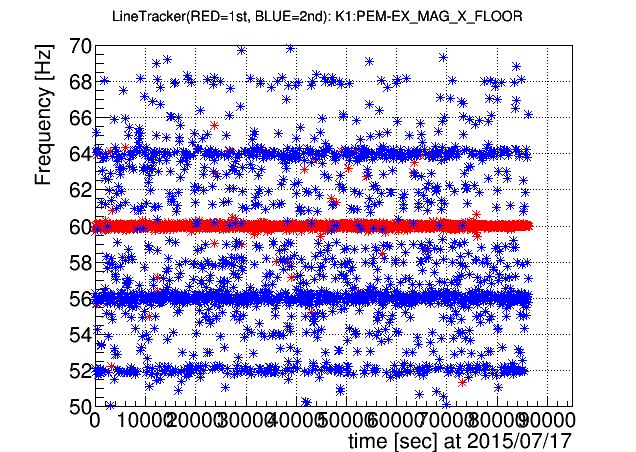
\includegraphics[width=0.9\hsize]{fig/LineTrackingMon/sample_freq.png}
    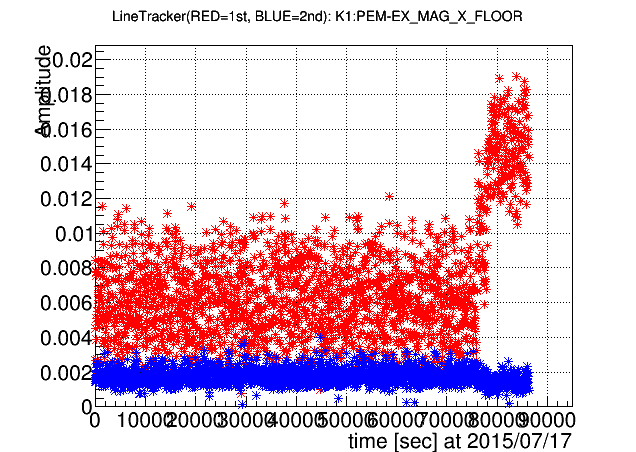
\includegraphics[width=0.9\hsize]{fig/LineTrackingMon/sample_amp.png}
    \caption{Sample plots of frequency (top) and amplitude (bottom) of a line obtained by LineTrackingMonitor. In this plot, nsig was set to 2, so only two signals (red and blue) are extracted. We show the strongest signal for each frame by red points and the second by blue. From the top panel, you can see the 60 Hz line was the strongest signal almost all the time. Also, you can see line-like signals every 4 Hz (i.e., $60 + 4m$ Hz, where $m \in \mathcal{Z}$). From the bottom panel, the amplitude of the 60 Hz line is found to have a large fluctuation (spread) and also there was a jump at around 80000 sec after the start of that day for unknown reasons.}
  \label{fig:nha_sample}
 \end{center}
\end{figure}

{\noindent \small contact person: Koh Ueno (\tt ueno@gwv.hep.osaka-cu.ac.jp)}

